% =============================================================================
% AMR Farbdesign - DIN A4 Querformat
% Build: xelatex farbdesign.tex
% =============================================================================
\documentclass[a4paper, landscape]{article}

% Erzwingt ein randloses DIN A4 Format (297mm x 210mm)
\usepackage[margin=0pt]{geometry}
\usepackage{tikz}
\usepackage{xcolor}
\usepackage{iftex}
\usepackage{hyperref}

% PDF direkt im Vollbildmodus oeffnen
\hypersetup{pdfpagemode=FullScreen}

% Schriftarten-Weiche (Fira Sans/Mono wenn mit XeLaTeX kompiliert)
\ifxetex
  \usepackage{fontspec}
  \setsansfont{Fira Sans}
  \setmonofont{Fira Mono}
\else
  \usepackage[T1]{fontenc}
  \renewcommand{\familydefault}{\sfdefault}
\fi

% Seitenzahlen ausblenden
\pagestyle{empty}

% Farbdefinitionen im HEX-Format
\definecolor{BgBase}{HTML}{0B131E}
\definecolor{BgPanel}{HTML}{111D2B}
\definecolor{TextSec}{HTML}{517C96}
\definecolor{AccPrim}{HTML}{00E5FF}
\definecolor{StatSucc}{HTML}{00FF66}
\definecolor{StatCrit}{HTML}{FF2A40}

\begin{document}%
\noindent%
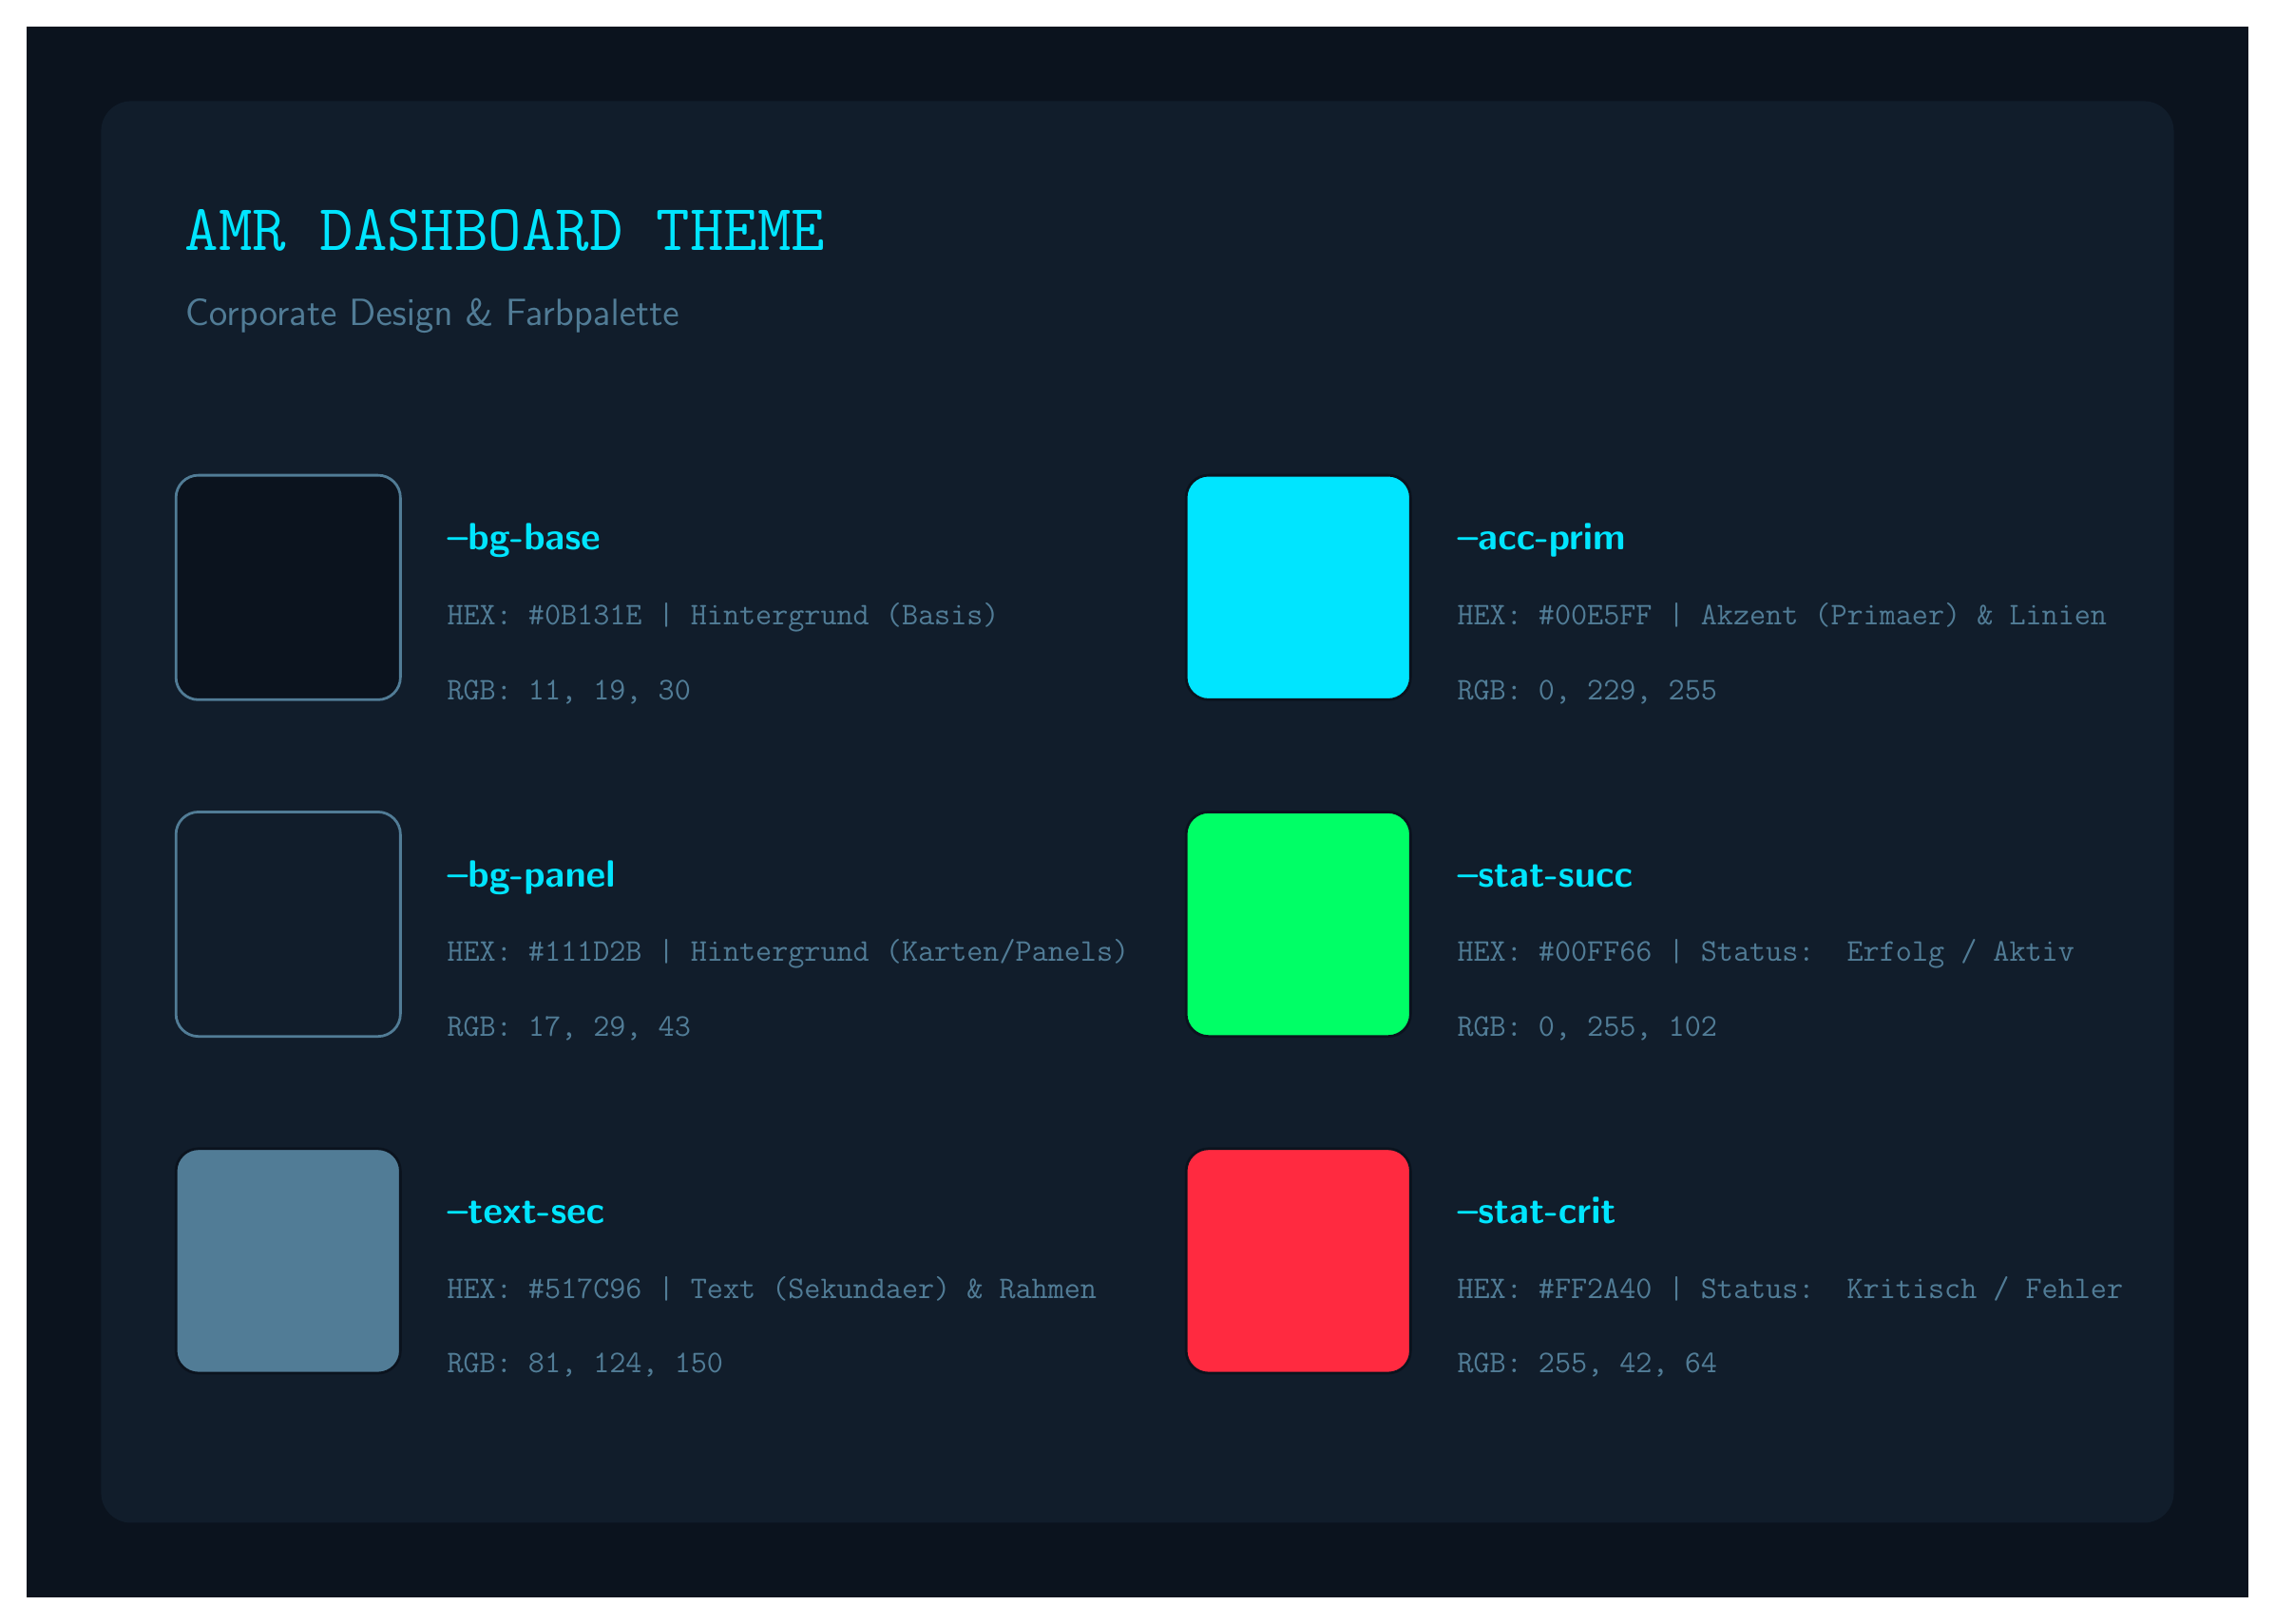
\begin{tikzpicture}[x=1mm, y=-1mm]

  % Container-Hintergruende (A4 Format exakt ausfuellen: 297 x 210 mm)
  \fill[BgBase] (0,0) rectangle (297,210);
  \fill[BgPanel, rounded corners=4mm] (10,10) rectangle (287,200);

  % Titel und Untertitel
  \node[anchor=base west, text=AccPrim, font=\ttfamily\bfseries\Huge] at (20,30) {AMR DASHBOARD THEME};
  \node[anchor=base west, text=TextSec, font=\sffamily\Large] at (20,40) {Corporate Design \& Farbpalette};

  % Makro fuer einheitliche Farbfelder (Grid-basiert)
  % Parameter: 1=x, 2=y, 3=Fill, 4=Stroke, 5=Var-Name, 6=Hex-Text, 7=RGB-Text
  \def\paletteentry#1#2#3#4#5#6#7{
    \begin{scope}[shift={(#1,#2)}]
      % Farbquadrat (30x30 mm)
      \filldraw[fill=#3, draw=#4, line width=1pt, rounded corners=3mm] (0,0) rectangle (30,30);
      % Textbeschriftungen rechts daneben
      \node[anchor=base west, text=AccPrim, font=\sffamily\bfseries\Large] at (35,10) {#5};
      \node[anchor=base west, text=TextSec, font=\ttfamily\large] at (35,20) {#6};
      \node[anchor=base west, text=TextSec, font=\ttfamily\large] at (35,30) {#7};
    \end{scope}
  }

  % Rendering der Paletten-Eintraege (2 Spalten, 3 Zeilen)

  % Spalte 1: x = 20
  \paletteentry{20}{60}{BgBase}{TextSec}{--bg-base}{HEX: \#0B131E | Hintergrund (Basis)}{RGB: 11, 19, 30}
  \paletteentry{20}{105}{BgPanel}{TextSec}{--bg-panel}{HEX: \#111D2B | Hintergrund (Karten/Panels)}{RGB: 17, 29, 43}
  \paletteentry{20}{150}{TextSec}{BgBase}{--text-sec}{HEX: \#517C96 | Text (Sekundaer) \& Rahmen}{RGB: 81, 124, 150}

  % Spalte 2: x = 155
  \paletteentry{155}{60}{AccPrim}{BgBase}{--acc-prim}{HEX: \#00E5FF | Akzent (Primaer) \& Linien}{RGB: 0, 229, 255}
  \paletteentry{155}{105}{StatSucc}{BgBase}{--stat-succ}{HEX: \#00FF66 | Status: Erfolg / Aktiv}{RGB: 0, 255, 102}
  \paletteentry{155}{150}{StatCrit}{BgBase}{--stat-crit}{HEX: \#FF2A40 | Status: Kritisch / Fehler}{RGB: 255, 42, 64}

\end{tikzpicture}%
\end{document}
